\documentclass[10pt,xcolor={dvipsnames}]{beamer}
\usetheme[
%%% option passed to the outer theme
%    progressstyle=fixedCircCnt,   % fixedCircCnt, movingCircCnt (moving is deault)
  ]{Feather}
  

% Change the background image on the title and final page.
% It stretches to fill the entire frame!
% \renewcommand{\backgroundfile}{example-grid-100x100pt}

%-------------------------------------------------------
% INCLUDE PACKAGES
%-------------------------------------------------------
\usepackage{amssymb}
\usepackage{tikz}
\usetikzlibrary{positioning}
\usetikzlibrary{shapes.arrows}
\usepackage{graphicx}
\usepackage{amsmath}
\usepackage[utf8]{inputenc}
\usepackage[english]{babel}
\usepackage[T1]{fontenc}
% \usepackage{helvet}

%% Load different font packages to use different fonts
%% e.g. using Linux Libertine, Linux Biolinum and Inconsolata
 \usepackage{libertine}
 \usepackage{zi4}

%%% e.g. using Carlito and Caladea
%\usepackage{carlito}
%\usepackage{caladea}
%\usepackage{zi4}

%% e.g. using Venturis ADF Serif and Sans
% \usepackage{venturis}

%-------------------------------------------------------
% DEFFINING AND REDEFINING COMMANDS
%-------------------------------------------------------

% colored hyperlinks
\newcommand{\chref}[2]{
  \href{#1}{{\usebeamercolor[bg]{Feather}#2}}
}
% Drawing Arrows
\tikzset{
    myarrowup/.style={
        draw,
        fill=ForestGreen,
        single arrow,
        minimum height=3.5ex,
        single arrow head extend=1ex}}

\tikzset{
    myarrowdown/.style={
        draw,
        fill=Red,
        single arrow,
        minimum height=3.5ex,
        single arrow head extend=1ex}}

\newcommand{\arrowup}{%
\tikz [baseline=-0.5ex]{\node [myarrowup,rotate=90] {};}
}
\newcommand{\arrowdown}{%
\tikz [baseline=-1ex]{\node [myarrowdown,rotate=-90] {};}
}

\newcommand\circledmark[1][Green!50]{%
  \tikz\node[circle,fill=#1,inner sep=0pt]{$\checkmark$};%
}

%-------------------------------------------------------
% INFORMATION IN THE TITLE PAGE
%-------------------------------------------------------

\title[Shiraz University]{
\includegraphics[width=0.5\textwidth]{Images/latex.png}} % The short title appears at the bottom of every slide, the full title is only on the title page
%\subtitle{Shiraz University}


\author{\textit{\textbf{Alireza Lotfi, Abdolrahim Touranian, Mohsen Tahmasbi}}}

\institute[Shiraz Universtiy] % Your institution as it will appear on the bottom of every slide, may be shorthand to save space
{
	Department of Computer Science, Engineering and IT \\
	Shiraz University % Your institution for the title page
}
\date{April 10, 2022}

%-------------------------------------------------------
% My commands and packages
%-------------------------------------------------------
\usepackage{multirow}
\usepackage{array}
\usepackage{academicons}
\usepackage{fontawesome}
\usepackage{pifont}
\usepackage{xcolor, colortbl}
\newcommand{\tac}{\centering\arraybackslash}


\definecolor{cadetgrey}{rgb}{0.57, 0.64, 0.69}
\definecolor{latexBird}{HTML}{008080}

% template
\setbeamertemplate{itemize item}{\ding{52}}

% Arrow up and down
\newcommand*\up{\textcolor{green}{%
		\ensuremath{\blacktriangle}}}
\newcommand*\down{\textcolor{red}{%
		\ensuremath{\blacktriangledown}}}
\newcommand*\const{\textcolor{darkgray}%
	{\textbf{--}}}

% emoji
\newcommand{\Simley}[1]{%
	\begin{tikzpicture}[scale=0.11]
		\newcommand*{\SmileyRadius}{1.0}%
		\draw [fill=brown!10] (0,0) circle (\SmileyRadius)% outside circle
		%node [yshift=-0.22*\SmileyRadius cm] {\tiny #1}% uncomment this to see the smile factor
		;  
		
		\pgfmathsetmacro{\eyeX}{0.5*\SmileyRadius*cos(30)}
		\pgfmathsetmacro{\eyeY}{0.5*\SmileyRadius*sin(30)}
		\draw [fill=cyan,draw=none] (\eyeX,\eyeY) circle (0.15cm);
		\draw [fill=cyan,draw=none] (-\eyeX,\eyeY) circle (0.15cm);
		
		\pgfmathsetmacro{\xScale}{2*\eyeX/180}
		\pgfmathsetmacro{\yScale}{1.0*\eyeY}
		\draw[color=red, domain=-\eyeX:\eyeX]   
		plot ({\x},{
			-0.1+#1*0.15 % shift the smiley as smile decreases
			-#1*1.75*\yScale*(sin((\x+\eyeX)/\xScale))-\eyeY});
	\end{tikzpicture}%
}


% fonts used
\usepackage{fontspec}
\setromanfont{EBGaramond}[
Path= Fonts/EBGaramond/,
Extension = .ttf,
UprightFont=*-Regular,
BoldFont=*-Bold,
ItalicFont=*-Italic,
BoldItalicFont=*-BoldItalic,
]

\setsansfont{EBGaramond}[
Path= Fonts/EBGaramond/,
Extension = .ttf,
UprightFont=*-Regular,
BoldFont=*-Bold,
ItalicFont=*-Italic,
BoldItalicFont=*-BoldItalic
]

\setmonofont{EBGaramond}[
Path= Fonts/EBGaramond/,
Extension = .ttf,
UprightFont=*-Regular,
BoldFont=*-Bold,
ItalicFont=*-Italic,
BoldItalicFont=*-BoldItalic
]

% different modes of effects
%\pause, \only, \visible \uncover or \onslide

%-------------------------------------------------------
% THE BODY OF THE PRESENTATION
%-------------------------------------------------------

\setbeamercolor{background canvas}{bg=latexBird!5}
\begin{document}

%-------------------------------------------------------
% THE TITLEPAGE
%-------------------------------------------------------

\begin{frame}[plain,noframenumbering] % the plain option removes the header from the title page, noframenumbering removes the numbering of this frame only
  \titlepage % call the title page information from above
\end{frame}

\begin{frame}{Overview}
	\tableofcontents
\end{frame}

%-------------------------------------------------------
\section{Introduction}
	
	\begin{frame}[plain,noframenumbering]
		\finalpage{\textcolor{beamer@normaltextcolor}{\LARGE\textbf{Introduction}}}
	\end{frame}

	\subsection{History}
		\begin{frame}{History}
			\pause
					
			\begin{columns}[T] % align columns
				\begin{column}{.65\textwidth}
					\onslide<2->
					~\\~\\\textbf{\color{beamer@headercolor}\TeX}, is a typesetting system which was designed and written by \textbf{\color{beamer@headercolor}Donald Knuth}, 
					a Stanford University professor, and first released in \textbf{\color{beamer@headercolor}1978}, to improve the quality of mathematical notation in his books.\newline \newline \newline \newline
					
					\onslide<3->
					\textbf{\color{beamer@headercolor}\LaTeX} is a software system for document preparation which was created in the early 
					\textbf{\color{beamer@headercolor}1980s} by \textbf{\color{beamer@headercolor}Leslie Lamport}, when he was working at SRI. 
					He needed to write TeX macros for his own use, and thought that with a little extra effort he could make a general package usable by others
				\end{column}%
				\hfill%
				\onslide<2->
				\begin{column}{.35\textwidth}
					\onslide<2->
					\begin{figure}
						\begin{tikzpicture}
							\begin{scope}[yshift=2]
								\clip [rounded corners=1cm] (0,0) rectangle coordinate (centerpoint) (3,3cm); 
								\node [inner sep=0pt] at (centerpoint) {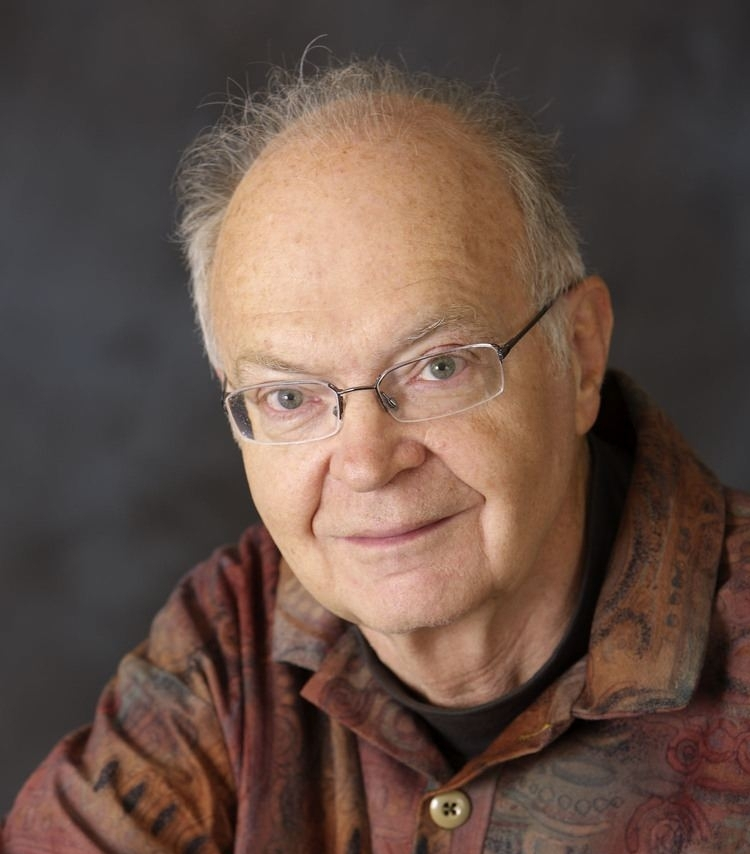
\includegraphics[width=3cm]{Images/donaldKnuth.jpeg}}; 
							\end{scope}
						\end{tikzpicture}
					\end{figure}
					\onslide<3->
					\begin{figure}
						\begin{tikzpicture}
							\begin{scope}[yshift=2]
								\clip [rounded corners=1cm] (0,0) rectangle coordinate (centerpoint) (3,3cm); 
								\node [inner sep=0pt] at (centerpoint) {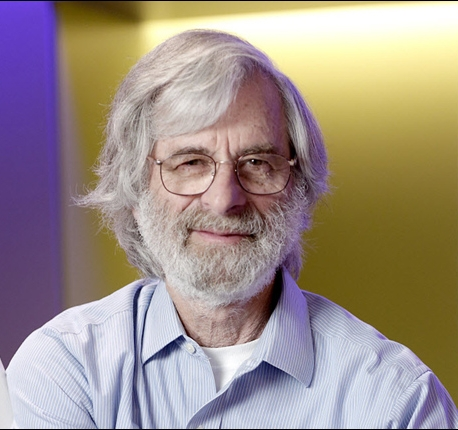
\includegraphics[width=4cm]{Images/lamport.jpg}}; 
							\end{scope}
						\end{tikzpicture}
					\end{figure}	
				\end{column}%
			\end{columns}
		
		\end{frame}
	
	\subsection{Comparison}
		\begin{frame}{MSWord vs \LaTeX}
			\pause
			
			\begin{center}
				\begin{tikzpicture}[line width=.1mm,rounded corners=.5em]
					
					\node (table) [clip,inner sep=.7\pgflinewidth] {
						\color{beamer@normaltextcolor} % text color
						\begin{tabular}[c]{>{\tac}m{5cm}|>{\tac}m{5cm}}
							\arrayrulecolor{beamer@headercolor}
							
							\cellcolor{beamer@headercolor}\color{white}MS Word & \cellcolor{beamer@headercolor}\color{white}\LaTeX \pause \\ 
							
							\rowcolor{cadetgrey!30}							
							Easy to use & Some hours to learn it \pause \\
							
							Useful for daily use & Technical \& Scientific work \pause \\ 
							
							\rowcolor{cadetgrey!30}							
							You have to pay for it & It is Free and Open source \pause \\
							
							Difficult citation management & Bibliography \pause \\ 
							
							\rowcolor{cadetgrey!30}							
							Difficult to change & Easy to change \pause \\
							
							What you see is what you get & Needs to be compiled \pause \\ 
							
							\rowcolor{cadetgrey!30}							
							Slow for large files & Faster because you write down only the contents \pause \\
							
							Useful for simple editing & Great mathematical tools \pause \\ 
							
							\rowcolor{cadetgrey!30}							
							Not compatible with all versions & Compatible (PDF output) \\
						
						\end{tabular}
					};
					\draw [rounded corners=.5em] (table.north west) rectangle (table.south east);
			\end{tikzpicture}
			\end{center}
 		\end{frame}
 	
 	\subsection{Start using}
	 	\begin{frame}{Applications}
	 		
	 		\begin{enumerate}[<+->]%[<+-| alert@+>]
	 			\onslide<2->
	 			\item Create graphic elements using \textbf{\color{beamer@headercolor}TikZ}
	 			\onslide<3->
	 			\item Create presentation slides with \textbf{\color{beamer@headercolor}Beamer} (Like our presentation \Simley{0.5})
	 		\end{enumerate}
	 		
	 		\onslide<2->
	 		\begin{columns}
	 			\begin{column}[c]{0.55\textwidth}
	 				\begin{figure}
	 					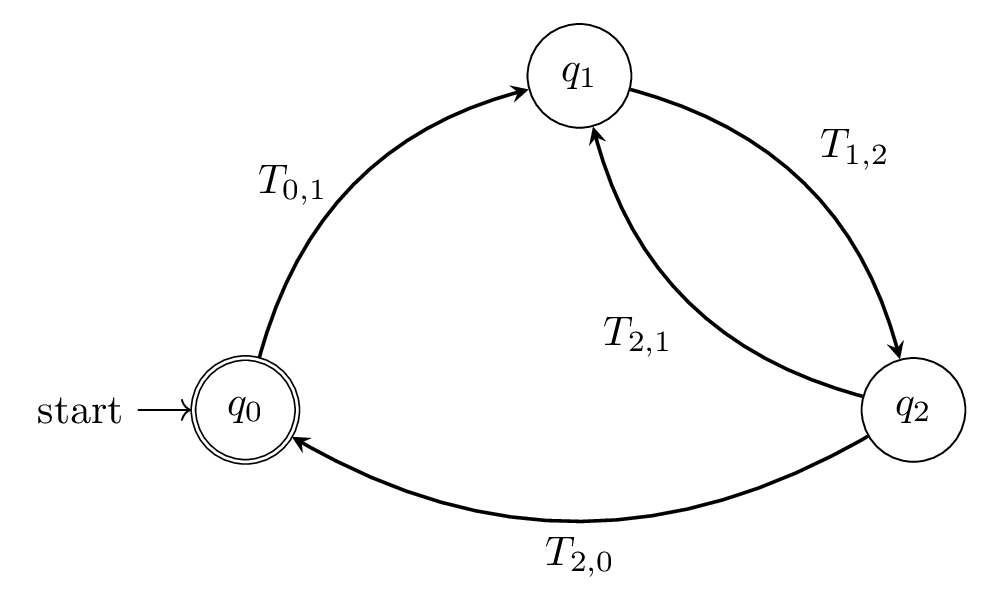
\includegraphics[width=0.75\linewidth]{Images/tikzSimple.png}
	 					\caption{Simple}
	 				\end{figure}
	 			\end{column}
	 			\hfill
	 			\begin{column}[c]{0.45\textwidth}
	 				\begin{figure}
	 					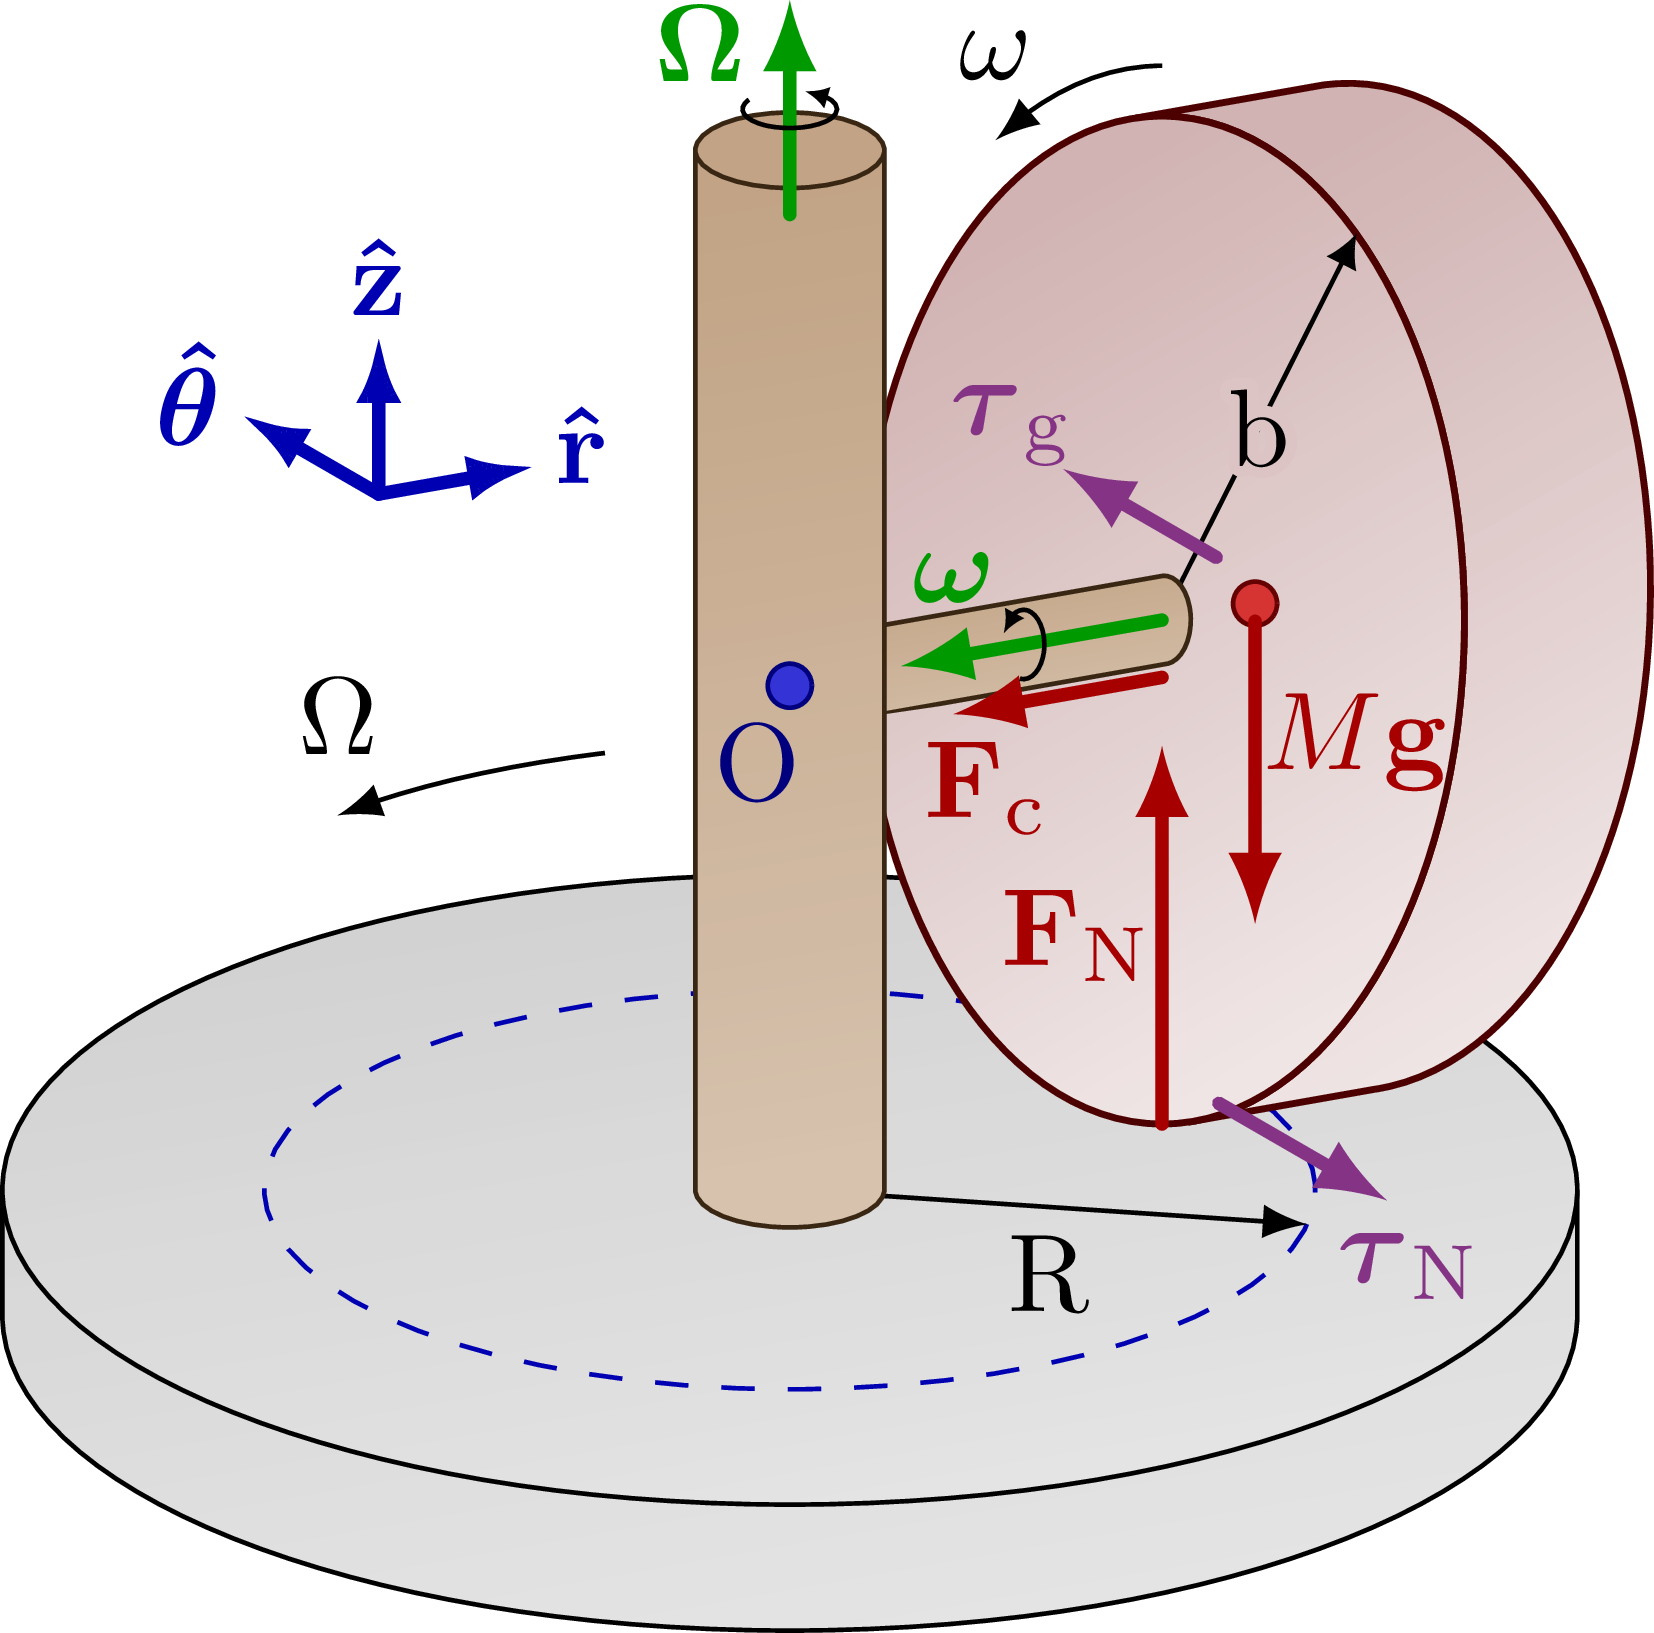
\includegraphics[width=0.75\linewidth]{Images/tikzHard.png}
	 					\caption{Complex}
	 				\end{figure}
	 			\end{column}
	 		\end{columns}
	 		
	 	\end{frame}
 	
 		\begin{frame}{Start using \LaTeX}

 			\begin{columns}[T]
 				\begin{column}{.7 \textwidth}
 					\onslide<2->
 					\textbf{Online platforms:}
 					\begin{itemize}[<+->]
 						\item<3-> \href{https://www.overleaf.com/learn/latex/Tutorials}{\textit{Overleaf (Recommended)}} 
 						\item<4-> \href{https://texlive.net/run}{\textit{Texlive}} 
 						\item<5-> \href{https://www.tutorialspoint.com/online_latex_editor.php}{\textit{Tutorialspoint}} 
 					\end{itemize}
 					
 					\vspace{1cm}
 					\onslide<6->
 					\textbf{Offline platforms:}
 					\begin{itemize}[<+->]
 						\onslide<7->
 						\item \textit{WinEdt + MiKTeX}
 						\onslide<8->
 						\item \textit{Texstudio + Tex Live } 
 					\end{itemize}

 				\end{column}
 			
 				\begin{column}{.3 \textwidth}
 					\onslide<7->
 					
\includegraphics[width=0.5\textwidth]{Images/windows.png}\vspace{1cm}
 					\onslide<8->
 					
\includegraphics[width=0.5\textwidth]{Images/linux.png}
 				\end{column}
 				
 			\end{columns}	
 			
 		\end{frame}
 	
 		\begin{frame}{Compile}
 			\onslide<2->
 			\textbf{\textit{English documents}} can be compiled using the procedure bellow:
 			\begin{enumerate}
 				\item<3-> Create a {\color{blue}[filename].tex} file
 				\item<4-> Write your program
 				\item<5-> Compile using {\color{red}\$} PDFLaTeX {\color{blue}[filename].tex}
	 		\end{enumerate}
 			
 			\vspace{1cm}
 			
 			\onslide<6->
 			\textbf{\textit{Persian documents}} can be compiled using the procedure bellow:
 			\begin{enumerate}
 				\item<7-> Create a {\color{blue}[filename].tex} file
 				\item<8-> Write your program
 				\item<9-> Compile using {\color{red}\$} XeLaTeX {\color{blue}[filename].tex}
 			\end{enumerate}
	 	\end{frame}
 		

\section{Basic Concepts}
	\begin{frame}[plain,noframenumbering]
		\finalpage{\textcolor{beamer@normaltextcolor}{\LARGE\textbf{Basic Concepts}}}
	\end{frame}

	\subsection{Overall structure of \TeX ~file}
	
	
		\begin{frame}{Overall structure of \TeX file}
			
			\begin{columns}[T]
				\begin{column}{.5 \textwidth}
					
					\onslide<2->
					\begin{block}{Standard Control Sequences}
						\textbackslash documentclass[{\color{red}options}]\{{\color{orange}class}\}\\
						\textbackslash usepackage\{{\color{blue}packages}\}\\
						\textbackslash begin\{document\}\\
						\quad......\\
						\textbackslash end\{document\}\\
					\end{block}
					
					
					\onslide<3->
					\begin{block}{Other Classes}
						\{report\}, \{book\}, \{letter\}, \{beamer\}, ...
					\end{block}
					
				\end{column}
				
				\onslide<4->
				\begin{column}{.5 \textwidth}
					\begin{example}
						\textbackslash documentclass[{\color{red}12pt}]\{{\color{orange}article}\}\\
						\textbackslash usepackage\{{\color{blue}tabularx,graphics}\}\\
						\textbackslash begin\{document\}\\
						\quad Hello world!\\
						\textbackslash newpage\\
						\quad Seems good using \LaTeX!\\
						\textbackslash end\{document\}\\
					\end{example}
				\end{column}
				
			\end{columns}

		\end{frame}
	
		\begin{frame}{Persian documents}
			\onslide<2->
			In order to write our documents in persian, we should use the 
			\href{http://ftp.lyx.org/pub/tex-archive/macros/xetex/latex/xepersian/xepersian.pdf}{\underline{\textit{XePersian package}}}. \\
			
			\begin{columns}[T]
				\onslide<3->
				\begin{column}{0.5 \textwidth}
					\begin{block}{Typesetting}
						\textbackslash documentclass\{{\color{blue}article}\}\\
						\textbackslash usepackage\{{\color{orange}xepersian}\}\\
						{\color{orange} \textbackslash settextfont\{XB Niloofar\}}\\
						\textbackslash begin\{{\color{blue}document}\}\\
						
						\quad 
\includegraphics[width=0.5\textwidth]{Files/persian.pdf}
						
						\textbackslash end\{{\color{blue}document}\}
						
					\end{block}
				\end{column}
				
				\onslide<4->
				\begin{column}{0.5 \textwidth}
					\vspace{1.5cm}
					
\includegraphics[width=1\textwidth]{Images/persian2.png}
				\end{column}
			\end{columns}
		\end{frame}
	
		\begin{frame}{Document info}
			\onslide<2->
			
			\begin{columns}[T]
				
				\begin{column}{.5 \textwidth}
					
					\onslide<2->
					\begin{block}{Typesetting}
						\textbackslash documentclass\{{\color{blue}article}\}\\
						{\color{orange}\textbackslash title}\{Just see how great is \LaTeX\}\\
						{\color{orange}\textbackslash author}\{Alireza Lotfi\}\\
						{\color{orange}\textbackslash date}\{\textbackslash today\}\\
						
						\textbackslash begin\{{\color{blue}document}\}\\
						\quad \textbackslash maketitle\\
						\textbackslash end\{{\color{blue}document}\}\\
					\end{block}	
				\end{column}
			
				\onslide<3->
				\begin{column}{.5 \textwidth}
					\vspace{1cm}
					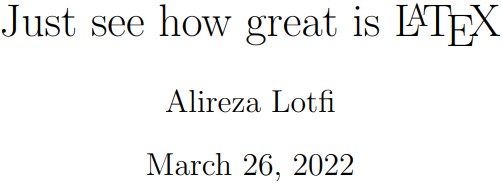
\includegraphics[width=1\textwidth]{Images/documentInfo.png}
				\end{column}

			\end{columns}
			
		\end{frame}
	
	\subsection{Section commands}
	
		\begin{frame}{Section , subsection, subsubsection}
			\begin{columns}[T]
				
				\begin{column}{.5 \textwidth}
					
					\onslide<2->
					\begin{block}{Typesetting}
						\textbackslash documentclass\{{\color{blue}article}\}\\
						
						\textbackslash begin\{{\color{blue}document}\}\\
						
						\quad  {\color{orange}\textbackslash section} \{name1\} \\
						\quad Testing section\\
						
						\quad\quad {\color{orange}\textbackslash subsection} \{name2\} \\
						\quad\quad Testing subsection\\
						
						\quad\quad\quad {\color{orange}\textbackslash subsubsection} \{name3\} \\
						\quad\quad\quad Testing subsubsection\\
						
						\quad\quad\quad\quad {\color{orange}\textbackslash paragraph} \{name4\} \\
						\quad\quad\quad\quad Testing paragraph\\
						
						\quad\quad\quad\quad\quad {\color{orange}\textbackslash subparagraph} \{name5\} \\
						\quad\quad\quad\quad\quad Testing subparagraph\\
						
						\textbackslash end\{{\color{blue}document}\}
					\end{block}	
				\end{column}
				
				\onslide<3->
				\begin{column}{.5 \textwidth}
					\vspace{0.75cm}
					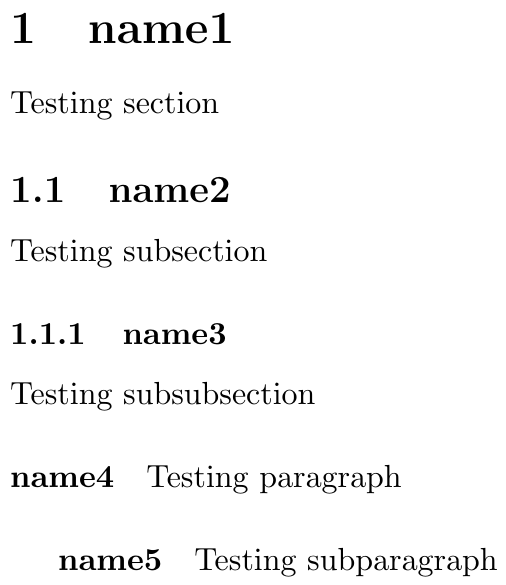
\includegraphics[width=1\textwidth]{Images/sections.png}
				\end{column}
				
			\end{columns}
		\end{frame}
	
		\begin{frame}{Table of contents}
			\onslide<2->
			Table of contents will be automatically created using the syntax bellow.\\
			
			\begin{columns}[T]
				\begin{column}{.4 \textwidth}
					
					\onslide<3->
					\begin{block}{Typesetting}
						\textbackslash documentclass\{{\color{blue}article}\}\\
						
						\textbackslash begin\{{\color{blue}document}\}\\
						
						\quad {\color{orange} \textbackslash tableofcontents}\\
						\quad {\color{orange} \textbackslash newpage}
						
						\textbackslash end\{{\color{blue}document}\}
						
					\end{block}	
				\end{column}
				
				\onslide<4->
				\begin{column}{.6 \textwidth}
					\vspace{1cm}
					\includegraphics[width=1\textwidth]{Images/tableofcontents.png}
				\end{column}
			\end{columns}
		
		\end{frame}
	
		
		\begin{frame}{Line break, comment}
			\onslide<2->
			\begin{block}{Result}
				I am going to break the line here \\
				and here. \newline
				But you can't see what I have written bellow. Maybe you should check the comments \Simley{0.5}.
			\end{block}
			
			\onslide<3->
			\begin{block}{Typesetting}
				\textbackslash documentclass\{{\color{blue}article}\}\\
				
				\textbackslash begin\{{\color{blue}document}\}\\
				I am going to break the line here {\color{orange}\textbackslash \textbackslash} \\
				and here. {\color{orange}\textbackslash newline}\\
				But you can't see what I have written bellow. Maybe you should check the comments \Simley{0.5}.\\
				{\color{orange}\textbackslash \%} Congratulations!! You found the comment.
				
				\textbackslash end\{{\color{blue}document}\}
			\end{block}
		\end{frame}
	

\section{Fundamental Commands}
	\begin{frame}[plain,noframenumbering]
		\finalpage{\textcolor{beamer@normaltextcolor}{\LARGE\textbf{Fundamental Commands}}}
	\end{frame}

	\subsection{Text decorations}
		\begin{frame}{Font size}
			
			\begin{columns}[T]
				
				\begin{column}{.5 \textwidth}
					\onslide<2->
					\begin{block}{Result}
						\tiny This is tiny.\\
						\scriptsize This is  scriptsize.\\
						\footnotesize This is footnotesize.\\
						\small This is small.\\
						\normalsize This is	normal size.\\
						\large This is large.\\
						\Large This is Large.\\
						\LARGE This is LARGE.\\
						\huge This is huge.\\
						\Huge This is Huge.\\
					\end{block}
				\end{column}
			
				\begin{column}{.5 \textwidth}
					\onslide<3->
					\begin{block}{Typesetting}
						\textbackslash documentclass\{{\color{blue}article}\}\\
						
						\textbackslash begin\{{\color{blue}document}\}\\
						
							\quad{\color{orange}\textbackslash tiny} This is tiny.\\
							\quad{\color{orange}\textbackslash scriptsize} This is scriptsize.\\
							\quad{\color{orange}\textbackslash footnotesize} This is footnotesize.\\
							\quad{\color{orange}\textbackslash small} This is small.\\
							\quad{\color{orange}\textbackslash normalsize} This is normal size.\\
							\quad{\color{orange}\textbackslash large} This is large.\\
							\quad{\color{orange}\textbackslash Large} This is Large.\\
							\quad{\color{orange}\textbackslash LARGE} This is LARGE.\\
							\quad{\color{orange}\textbackslash huge} This is huge.\\
							\quad{\color{orange}\textbackslash Huge} This is Huge.\\
						
						\textbackslash end\{{\color{blue}document}\}
					\end{block}
				\end{column}
			
			\end{columns}

		\end{frame}
		
		\begin{frame}{Font styles}
			\onslide<2->
			\begin{block}{Result}
				Do not \textit{worry about} your \textbf{difficulties} in \underline{mathematic},
				I assure you that mine are \huge greater. \normalsize

				\begin{flushright}
					\underline{\textbf{\textit{Einstein, Albert}}} (1879-1955)
				\end{flushright}
			\end{block}
			
			\onslide<3->
			\begin{block}{Typesetting}
				Do not {\color{orange}\textbackslash textit\{}worry about{\color{orange}\}} your {\color{orange}\textbackslash textbf\{}difficulties{\color{orange}\}} 
				in {\color{orange}\textbackslash underline\{}mathematic{\color{orange}\}},
				I assure you that mine are \textbackslash huge greater \textbackslash normalsize.\\
				
				\% You don't need to know what is flushright!\\  
				\textbackslash begin\{flushright\}\\
				\quad {\color{orange}\textbackslash underline\{\textbackslash textbf\{\textbackslash textit\{}Einstein, Albert{\color{orange}\}\}\}} (1879-1955)\\
				\textbackslash end\{flushright\}\\
				
			\end{block}
		\end{frame}
	
	\subsection{Lists and tables}
		\begin{frame}{Ordered list}
			\begin{columns}[T]
				
				\begin{column}{.5 \textwidth}
					\onslide<2->
					\begin{block}{Typesetting}
						\textbackslash documentclass\{{\color{blue}article}\}\\
						
						\textbackslash begin\{{\color{blue}document}\}\\
						
							\quad\textbackslash begin\{{\color{orange}enumerate}\}\\
								\qquad {\color{orange}\textbackslash item} First item\\
								\qquad {\color{orange}\textbackslash item} Second item\\
								\qquad {\color{orange}\textbackslash item} Third item\\
							\quad\textbackslash end\{{\color{orange}enumerate}\}\\

						\textbackslash end\{{\color{blue}document}\}
					\end{block}
				\end{column}
				
				\begin{column}{.5 \textwidth}
					\onslide<3->
					\begin{block}{Result}
						\begin{enumerate}
							\item First item
							\item Second item
							\item Third item
						\end{enumerate}
					\end{block}
				\end{column}
				
			\end{columns}
		\end{frame}
	
		\begin{frame}{Unordered list}
			\begin{columns}[T]
				
				\begin{column}{.5 \textwidth}
					\onslide<2->
					\begin{block}{Typesetting}
						\textbackslash documentclass\{{\color{blue}article}\}\\
						
						\textbackslash begin\{{\color{blue}document}\}\\
						
							\quad\textbackslash begin\{{\color{orange}itemize}\}\\
								\qquad {\color{orange}\textbackslash item} First item\\
								\qquad {\color{orange}\textbackslash item} Second item\\
								\qquad {\color{orange}\textbackslash item} Third item\\
							\quad\textbackslash end\{{\color{orange}itemize}\}\\
						
						\textbackslash end\{{\color{blue}document}\}
					\end{block}
				\end{column}
				
				\begin{column}{.5 \textwidth}
					\onslide<3->
					\begin{block}{Result}
						\begin{itemize}
							\item First item
							\item Second item
							\item Third item
						\end{itemize}
					\end{block}
				\end{column}
				
			\end{columns}
		\end{frame}
	
		\begin{frame}{Nested lists}
			\begin{columns}[T]
				
				\begin{column}{.5 \textwidth}
					\onslide<2->
					\begin{block}{Typesetting}
						\textbackslash documentclass\{{\color{blue}article}\}\\
						
						\textbackslash begin\{{\color{blue}document}\}\\
						
						\quad \textbackslash begin\{{\color{orange}enumerate}\}\\
							\qquad {\color{orange}\textbackslash item} First item\\
							
								\quad\qquad \textbackslash begin\{{\color{orange}itemize}\}\\
								\qquad\qquad {\color{orange}\textbackslash item} First nested item\\
								\qquad\qquad {\color{orange}\textbackslash item} Second nested item\\
								\quad\qquad \textbackslash end\{{\color{orange}itemize}\}\\
							
							\qquad {\color{orange}\textbackslash item} Second item\\
							\qquad {\color{orange}\textbackslash item} Third item\\
						\quad \textbackslash end\{{\color{orange}enumerate}\}\\
						
						\textbackslash end\{{\color{blue}document}\}
					\end{block}
				\end{column}
				
				\begin{column}{.5 \textwidth}
					\onslide<3->
					\begin{block}{Result}
						\begin{enumerate}
							\item First item
							\begin{itemize}
								\item First nested item
								\item Second nested item
							\end{itemize}
							\item Second item
							\item Third item
						\end{enumerate}
					\end{block}
				\end{column}
				
			\end{columns}
		\end{frame}
	
		\begin{frame}{Simple table}
			\begin{columns}[T]
				
				\begin{column}{.6 \textwidth}
					\onslide<2->
					\begin{block}{Typesetting}
						\textbackslash documentclass\{{\color{blue}article}\}\\
						
						\textbackslash begin\{{\color{blue}document}\}\\
						
							\quad\textbackslash begin\{{\color{orange}tabular}\}{\color{orange}\{c||c|c\}}\\
								\qquad Function {\color{orange}\&} X {\color{orange}\&} Y {\color{orange}\textbackslash \textbackslash \textbackslash hline} \\
								\qquad f(x, y) {\color{orange}\&} 10 {\color{orange}\&} 11 {\color{orange}\textbackslash \textbackslash}\\
								\qquad z(x, y) {\color{orange}\&} 12 {\color{orange}\&} 13 {\color{orange}\textbackslash \textbackslash}\\
								\qquad w(x, y) {\color{orange}\&} 14 {\color{orange}\&} 15 {\color{orange}\textbackslash \textbackslash}\\
							\quad\textbackslash end\{{\color{orange}tabular}\}\\
						
						\quad\textbackslash end\{{\color{blue}document}\}
					\end{block}
				\end{column}
				
				\begin{column}{.4 \textwidth}
					\onslide<3->
					\begin{block}{Result}
						\begin{tabular}{c||c|c}
							Function & X & Y \\ \hline
							f(x, y) & 10 & 11\\
							z(x, y) & 12 & 13\\
							w(x, y) & 14 & 15 \\
						\end{tabular}	
					\end{block}
				\end{column}
				
			\end{columns}
			
		\end{frame}
	
		\begin{frame}{Positioning table}
				\begin{columns}[T]
					
					\begin{column}{.6 \textwidth}
						\onslide<2->
						\begin{block}{Typesetting}
							\textbackslash documentclass\{{\color{blue}article}\}\\
							
							\textbackslash begin\{{\color{blue}document}\}\\
								\quad\textbackslash begin\{{\color{orange}table}\}{\color{orange}[h]}\\
									\qquad\textbackslash centering\\
									\qquad\textbackslash begin\{{\color{orange}tabular}\}{\color{orange}\{c||c|c\}}\\
										\quad\qquad Function {\color{orange}\&} X {\color{orange}\&} Y {\color{orange}\textbackslash \textbackslash \textbackslash hline} \\
										\quad\qquad f{x, y} {\color{orange}\&} 10 {\color{orange}\&} 11 {\color{orange}\textbackslash \textbackslash}\\
										\quad\qquad z(x, y) {\color{orange}\&} 12 {\color{orange}\&} 13 {\color{orange}\textbackslash \textbackslash}\\
										\quad\qquad w(x, y) {\color{orange}\&} 14 {\color{orange}\&} 15 {\color{orange}\textbackslash \textbackslash}\\
									\qquad\textbackslash end\{{\color{orange}tabular}\}\\
									\qquad{\color{orange}\textbackslash caption\{}This is our table{\color{orange}\}}\\
									\qquad{\color{orange}\textbackslash label\{}table\_ref\_1{\color{orange}\}}\\
								\quad\textbackslash begin\{{\color{orange}table}\}\\
								
								
							\textbackslash end\{{\color{blue}document}\}
						\end{block}
					\end{column}
					
					\begin{column}{.4 \textwidth}
						\onslide<3->
						\begin{block}{Result}
							\begin{table}[h]
								\centering
								\begin{tabular}{c||c|c}
									Function & X & Y \\ \hline
									f(x, y) & 10 & 11\\
									z(x, y) & 12 & 13\\
									w(x, y) & 14 & 15 \\
								\end{tabular}
							\caption{This is our table}
							\label{table_ref_1}
							\end{table}
						\end{block}
					\end{column}
					
				\end{columns}
			
		\end{frame}
	
	
	\subsection{Mathematical notations}
		\begin{frame}{Mathematical modes}
			
			\onslide<2->
			You can use any of these "delimiters" to typeset your math in \textbf{\underline{inline mode}}:\\
			\begin{itemize}
				\item<3-> {\color{orange}\textbackslash(}...{\color{orange}\textbackslash)}
				\item<4-> {\color{orange}\$}...{\color{orange}\$}
				\item<5-> \textbackslash begin\{{\color{orange}math}\}...\textbackslash end\{{\color{orange}math}\}
			\end{itemize}
			
			\vspace{1cm}
			\onslide<6->
			Use one of these constructions to typeset maths in \textbf{\underline{display mode:}}\\
			\begin{itemize}
				\item<7-> {\color{orange}\textbackslash[}...{\color{orange}\textbackslash]}
				\item<8-> \textbackslash begin\{{\color{orange}displaymath}\}...\textbackslash end\{{\color{orange}displaymath}\}
				\item<9-> \textbackslash begin\{{\color{orange}equation}\}...\textbackslash end\{{\color{orange}equation}\}
			\end{itemize}
		
		\end{frame}
	
		\begin{frame}{Inline mode example}
			
			\onslide<2->
			\begin{block}{Typesetting}
				\textbackslash documentclass\{{\color{blue}article}\}\\
				
				\textbackslash begin\{{\color{blue}document}\}\\
				
				\quad Ex 1: {\color{orange}\textbackslash(}f(x) = 2\textbackslash times x + 5{\color{orange}\textbackslash)} \textbackslash\textbackslash\\
				
				\quad Ex 2: {\color{orange}\$}f(x) = 2\textbackslash times x + 5{\color{orange}\$} \textbackslash\textbackslash\\
				
				\quad Ex 3: \textbackslash begin\{{\color{orange}math}\}f(x) = 2\textbackslash times x + 5 \textbackslash end\{{\color{orange}math}\}\\
				
				\textbackslash end\{{\color{blue}document}\}\\
			\end{block}
				
			\onslide<3->
			\begin{block}{Result}
				Ex 1: \(f(x) = 2\times x + 5\) \\
				Ex 2: $f(x) = 2\times x + 5$ \\
				Ex 3: \begin{math}	f(x) = 2\times x + 5 \end{math}
			\end{block}
			
		\end{frame}
	
		\begin{frame}{Display mode example}
			
			\begin{minipage}{.95\textwidth}
				\onslide<2->
				\begin{block}{Typesetting}
					\textbackslash documentclass\{{\color{blue}article}\}\\
					
					\textbackslash begin\{{\color{blue}document}\}\\
					
					\quad Ex 1: {\color{orange}\textbackslash[}f(x) = 2\textbackslash times x + 5{\color{orange}\textbackslash]} \textbackslash\textbackslash\\
					
					\quad Ex 2: \textbackslash begin\{{\color{orange}displaymath}\}f(x) = 2\textbackslash times x + 5 \textbackslash end\{{\color{orange}displaymath}\}\\
					
					\quad Ex 3: \textbackslash begin\{{\color{orange}equation}\}f(x) = 2\textbackslash times x + 5 \textbackslash end\{{\color{orange}equation}\}\\
					
					\textbackslash end\{{\color{blue}document}\}\\
				\end{block}
			\end{minipage}
			
			\begin{minipage}{.95 \textwidth}
				\onslide<3->
				\begin{block}{Result}
					Ex 1: \[f(x) = 2\times x + 5\] \\
					Ex 2: \begin{displaymath}	f(x) = 2\times x + 5 \end{displaymath}\\
					Ex 3: \begin{equation}	f(x) = 2\times x + 5 \end{equation}\\
				\end{block}
			\end{minipage}
		\end{frame}
	
	
		\begin{frame}{Subscripts and superscripts}
			\begin{columns}[T]
				\onslide<2->
				\begin{column}{.6\textwidth}
					\begin{block}{Typesetting}
						\textbackslash documentclass\{{\color{blue}article}\}\\
						
						\textbackslash begin\{{\color{blue}document}\}\\
							
							\quad Superscript: \textbackslash[f(x) = x{\color{orange}\textasciicircum\{}2+y{\color{orange}\}} + 5\textbackslash]\\
							\quad Subscript: \textbackslash[x{\color{orange}\_\{}n{\color{orange}\}} = x{\color{orange}\_\{}n-1{\color{orange}\}} 
							+ x{\color{orange}\_\{}n-2{\color{orange}\}}\textbackslash]\\
							
						\textbackslash end\{{\color{blue}document}\}\\
					\end{block}
				\end{column}
			
				\onslide<3->
				\begin{column}{.4\textwidth}
					\begin{block}{Result}
						Superscript: \[f(x) = x^{2+y} + 5\]
						Superscript: \[x_{n} = x_{n-1} + x_{n-2}\]
					\end{block}					
				\end{column}
			\end{columns}
		\end{frame}
	
	
		\begin{frame}{Basic operations}
			\pause
			\begin{center}
				\begin{tikzpicture}[line width=.1mm,rounded corners=.5em]
					
					\node (table) [clip,inner sep=.7\pgflinewidth] {
						\color{beamer@normaltextcolor} % text color
						\begin{tabular}[c]{>{\tac}m{5cm}|>{\tac\color{orange}}m{2cm}|>{\tac}m{2cm}}
							\arrayrulecolor{beamer@headercolor}
							
							\cellcolor{beamer@headercolor}\color{white}Description & \cellcolor{beamer@headercolor}\color{white}Command 
							& \cellcolor{beamer@headercolor}\color{white}Output\pause \\ 
							
							\rowcolor{cadetgrey!30}
							multiplication (times) & \textbackslash times & $\times$\pause\\
							
							multiplication (dot) & \textbackslash cdot & $\cdot$\pause\\
							
							\rowcolor{cadetgrey!30}
							division symbol & \textbackslash div & $\div$\pause\\
							
							division (slash) & / & $/$\pause\\
							
							\rowcolor{cadetgrey!30}
							fraction & \textbackslash frac\{a\}\{b\} & $\frac{a}{b}$\pause\\
							
							square root & \textbackslash sqrt\{x\} & $\sqrt{x}$\pause\\
							
							\rowcolor{cadetgrey!30}
							$n$th root & \textbackslash sqrt[n]\{x\} & $\sqrt[n]{x}$\pause\\
							
							exponentiation & \textbackslash a\textasciicircum b & $a^{b}$\pause\\
							
							\rowcolor{cadetgrey!30}
							natural log  & \textbackslash ln(x) & $\ln(x)$\pause\\
							
							logarithms & \textbackslash log\_\{a\}b & $\log_{a}b$\pause\\
							
							\rowcolor{cadetgrey!30}
							exponential function & e\textasciicircum x= \textbackslash exp(x) & $e^{x}=\exp(x)$\\
							
						\end{tabular}
					};
					\draw [rounded corners=.5em] (table.north west) rectangle (table.south east);
				\end{tikzpicture}
			\end{center}
		\end{frame}
	
	\subsection{URL and image insertion}
		\begin{frame}{URL and hyper ref}
			\begin{columns}[T]
				
				\begin{column}{.6 \textwidth}
					\onslide<2->
					\begin{block}{Typesetting}
						\textbackslash documentclass\{{\color{blue}article}\}\\
						\textbackslash usepackage\{{\color{orange}hyperref}\}\\
						\textbackslash begin\{{\color{blue}document}\}\\
							\quad{\color{orange}\textbackslash url\{}{\color{red}link}{\color{orange}\}}\\
							\quad{\color{orange}\textbackslash href\{}{\color{red}link}{\color{orange}\}\{}{\color{red}text}{\color{orange}\}}\\
						\textbackslash end\{{\color{blue}document}\}\\
					\end{block}
					
					\onslide<3->
					\begin{example}{Typesetting}
						\textbackslash documentclass\{{\color{blue}article}\}\\
						\textbackslash usepackage\{{\color{orange}hyperref}\}\\
						\textbackslash begin\{{\color{blue}document}\}\\
							\quad{\color{orange}\textbackslash url\{}https://google.com/{\color{orange}\}}\\
							\quad{\color{orange}\textbackslash href\{}https://google.com/{\color{orange}\}\{}Google{\color{orange}\}}\\
						\textbackslash end\{{\color{blue}document}\}\\
					\end{example}
				\end{column}
			
			
				\onslide<4->
				\begin{column}{.4 \textwidth}
					\vspace{2cm}
					\begin{block}{Result}
						\url{https://google.com}\\
						\href{https://google.com}{Google}
					\end{block}
				\end{column}
			\end{columns}
		
		\end{frame}
	
		\begin{frame}{Simple image}
			\begin{columns}[T]
				
				\begin{column}{.6 \textwidth}
					\onslide<2->
					\begin{block}{Typesetting}
						\textbackslash documentclass\{{\color{blue}article}\}\\
						\textbackslash usepackage\{{\color{orange}graphicx}\}\\
						\textbackslash begin\{{\color{blue}document}\}\\
							\quad{\color{orange}\textbackslash includegraphics\{[}{\color{red}Options}{\color{orange}]\{}{\color{red}File path}{\color{orange}\}\}}\\
						\textbackslash end\{{\color{blue}document}\}\\
					\end{block}
				\end{column}
				
				\onslide<4->
				\begin{column}{.4 \textwidth}
					\vspace{.5cm}
					\centering
					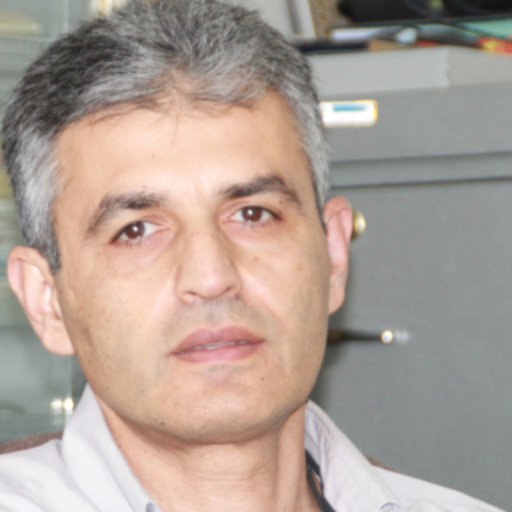
\includegraphics[width=0.6\textwidth]{Images/ziarati.jpg}
				\end{column}
			\end{columns}
		
			\onslide<3->
			\begin{example}
				\textbackslash documentclass\{{\color{blue}article}\}\\
				\textbackslash usepackage\{{\color{orange}graphicx}\}\\
				\textbackslash begin\{{\color{blue}document}\}\\
					\quad{\color{orange}\textbackslash includegraphics\{[}width=0.6 \textbackslash textwidth{\color{orange}]\{}Images/ziarati.jpg{\color{orange}\}\}}\\
				\textbackslash end\{{\color{blue}document}\}\\
			\end{example}
		
		\end{frame}
	
		\begin{frame}{Positioning image}
			\begin{minipage}{.95\textwidth}
				\onslide<2->
				\begin{block}{Typesetting}
					\textbackslash documentclass\{{\color{blue}article}\}\\
					\textbackslash usepackage\{{\color{orange}graphicx}\}\\
					\textbackslash begin\{{\color{blue}document}\}\\
						\quad\textbackslash begin\{{\color{orange}figure}\}[h]\\
							\qquad \textbackslash centering\\
							\qquad{\color{orange}\textbackslash includegraphics\{[}width=0.12 \textbackslash textwidth{\color{orange}]\{}Images/ziarati2.jpeg{\color{orange}\}\}}\\
							\qquad \textbackslash caption\{This is our image\}\\
							\qquad \textbackslash label\{image\_ref\_1\}\\
						\quad\textbackslash end\{{\color{orange}figure}\}\\
					\textbackslash end\{{\color{blue}document}\}\\
				\end{block}
			\end{minipage}
				
			\onslide<3->
			\begin{figure}[h]
				\centering
				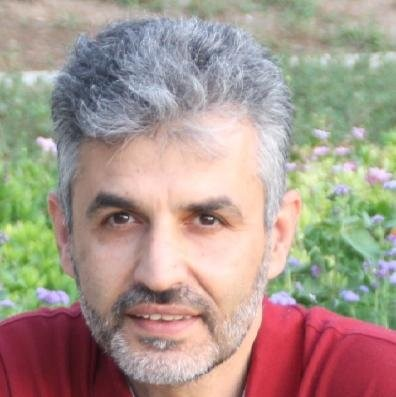
\includegraphics[width=0.12\textwidth]{Images/ziarati2.jpeg}
				\caption{This is our image}
				\label{image_ref_1}
			\end{figure}
			
		\end{frame}
	
	\subsection{Bibliography}
		\begin{frame}{Bibliography (thebibliography environment)}
	
			\begin{columns}[T]
				
				\begin{column}{.5 \textwidth}
					\onslide<2->
					\begin{block}{Typesetting}
						\textbackslash documentclass\{{\color{blue}article}\}\\
						\textbackslash begin\{{\color{blue}document}\}\\
							
							\quad\textbackslash begin\{{\color{orange}thebibliography}\}{\color{orange}\{maxItems\}}\\
								\qquad{\color{orange}\textbackslash bibitem\{}ref1{\color{orange}\}} item 1\\
								\qquad{\color{orange}\textbackslash bibitem\{}ref2{\color{orange}\}} item 2\\
							\quad\textbackslash end\{{\color{orange}thebibliography}\}\\
						
						\textbackslash end\{{\color{blue}document}\}\\
					\end{block}
				
					\onslide<4->
					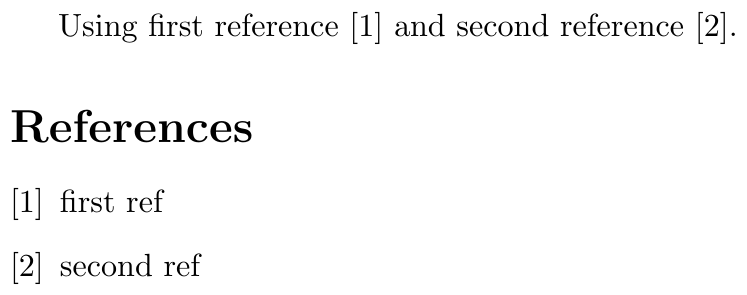
\includegraphics[width=1\textwidth]{Images/reference.png}
				\end{column}
				
				\onslide<3->
				\begin{column}{.5 \textwidth}
					\begin{example}
						\textbackslash documentclass\{{\color{blue}article}\}\\
						\textbackslash begin\{{\color{blue}document}\}\\
						
							\quad Using first reference {\color{orange}\textbackslash cite\{}first{\color{orange}\}} and \\
							\quad second reference {\color{orange}\textbackslash cite\{}second{\color{orange}\}}.\\
							\quad\textbackslash begin\{{\color{orange}thebibliography}\}{\color{orange}\{9\}}\\
								\qquad{\color{orange}\textbackslash bibitem\{}first{\color{orange}\}} first ref\\
								\qquad{\color{orange}\textbackslash bibitem\{}second{\color{orange}\}} second ref\\
							\quad\textbackslash end\{{\color{orange}thebibliography}\}\\
						
						\textbackslash end\{{\color{blue}document}\}\\
					\end{example}
					
				\end{column}
			\end{columns}
		
		\end{frame}
	
		\begin{frame}{Bibliography (bibtex)}
			\onslide<2->
			To use bibtex you must:
			\begin{enumerate}
				\item<3-> Create a database (.bib) file that describes the articles that you want to reference.
				\item<4-> Specify the style and location of the bibliography in your LaTeX document.
				\item<5-> Run latex and bibtex.
			\end{enumerate}
			
			\vspace{1cm}
			\onslide<6->
			Why should you use Bibtex?
			\begin{itemize}
				\item<7-> Let the style file worry about formatting the bibliography.
				\item<8-> Avoid retyping the same references for your next paper (even if it is for a journal with a completely difference bibliography style).
				\item<9-> It is more efficient.
				\item<10-> It is not hard!
			\end{itemize}

		\end{frame}
	
		\begin{frame}{Example bibliography database}
			
			\only<2>{\vspace{1cm}\centering
\includegraphics[width=1\textwidth]{Images/scholar_1.png}}
			\only<3>{\vspace{0.5cm}\centering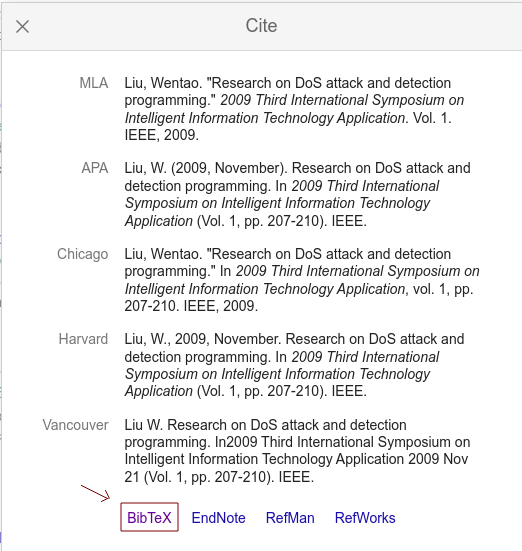
\includegraphics[width=.5\textwidth]{Images/scholar_2.png}}
			\only<4>{\vspace{1cm}\centering
\includegraphics[width=1\textwidth]{Images/scholar_3.png}}
			
		\end{frame}
	
		\begin{frame}{Example \LaTeX~file}
			\begin{columns}[T]
				
				\begin{column}{.5 \textwidth}
					\onslide<2->
					\begin{block}{Typesetting}
						\textbackslash documentclass\{{\color{blue}article}\}\\
						\textbackslash begin\{{\color{blue}document}\}\\
						
							\quad...\\
							\quad {\color{orange}\textbackslash bibliographystyle\{}style{\color{orange}\}}\\
							\quad {\color{orange}\textbackslash bibliography\{}.bib file name{\color{orange}\}}\\
						
						\textbackslash end\{{\color{blue}document}\}\\
					\end{block}
					
				\end{column}
				
				\onslide<3->
				\begin{column}{.5 \textwidth}
					\begin{example}
						\textbackslash documentclass\{{\color{blue}article}\}\\
						\textbackslash begin\{{\color{blue}document}\}\\
						
						\quad This reference {\color{orange}\textbackslash cite\{}liu2009research{\color{orange}\}}\\
						\quad is what we were talking about.\\
						\quad {\color{orange}\textbackslash bibliographystyle\{}plain{\color{orange}\}}\\
						\quad {\color{orange}\textbackslash bibliography\{}database{\color{orange}\}}\\
						
						\textbackslash end\{{\color{blue}document}\}\\
					\end{example}
					
				\end{column}
			\end{columns}
		
			\onslide<4->
			\vspace{.2cm}
			
\includegraphics[width=1\textwidth]{Images/reference2.png}
		\end{frame}


\section{References}
\begin{frame}{References}
	\begin{enumerate}
		\item \href{https://en.wikipedia.org/wiki/LaTeX}{\textit{\underline{https://en.wikipedia.org}}}
		\item \href{https://www.latex-project.org/get/}{\textit{\underline{https://www.latex-project.org}}}
		\item \href{https://www.overleaf.com/learn/latex/Tutorials?&nocdn=true}{\textit{\underline{https://www.overleaf.com}}}
		\item \href{https://www.learnlatex.org/en/}{\textit{\underline{https://www.learnlatex.org}}}
		\item \href{https://texlive.net/run}{\textit{\underline{https://texlive.net/run}}}
		\item \href{https://www.unf.edu/~wkloster/latex/bib.html}{\textit{\underline{https://www.unf.edu}}}
		\item \href{https://realtechnologytools.com/latex-template/}{\textit{\underline{https://realtechnologytools.com}}}
		\item \href{http://mirrors.ibiblio.org/CTAN/macros/xetex/latex/xepersian/xepersian-doc.pdf}{\textit{\underline{http://mirrors.ibiblio.org}}}
	\end{enumerate}
\end{frame}

		
\section{Live coding}
	\begin{frame}[plain,noframenumbering]
		\finalpage{\textcolor{beamer@normaltextcolor}{\LARGE\textbf{Live Coding}}}
	\end{frame}



\end{document} 